\documentclass[a4paper,10pt,print]{article}
\usepackage{mathrsfs}
\usepackage{fancyhdr}
\pagestyle{fancy}
\usepackage{verbatim}
\usepackage{graphicx}
%\usepackage{bbding}
\usepackage{booktabs}
\usepackage{multirow}
\usepackage{tabularx}
\usepackage{amsmath,amssymb}

\title{\textbf{Temperature Effect on Rubber Balloon}}
\author{
%Dingwen Wang\\
%Department of Astronautical Science and Engineering,\\
%School of Aerospace and Materials Engineering,\\
%National University of Defense Technology, Changsha, PR China\\
%wangdingwen0618@gmail.com
%\and Puyun Gao\\
%Department of Astronautical Science and Engineering,\\
%School of Aerospace and Materials Engineering,\\
%National University of Defense Technology, Changsha, PR China
}
\date{}
\begin{document}

\maketitle
\graphicspath{{Figures/}}

\begin{abstract}
The inflation of rubber balloon is realized by the pressure jump across the membrane.
The spherical balloon has a non-monotonic pressure-radius characteristic.
For rubber is material of entropy induced elasticity, the temperature effect should be considered when we refers to the deformation of rubber balloon in extreme environment.
In this paper, we want to find out how much of the effect on the performance of rubber balloon during the ascending process. The result shows that the temperature effect is not negligible when we use rubber balloon as High Altitude Long Duration(HALD)aerostat.
\\
\emph{Key words}: Rubber balloons, Mooney--Rivlin model, Temperature effect, HALD aerostat
\end{abstract}

  \section{Introduction}

Rubber balloon plays an important role in scientific activities, such as high altitude atmosphere research, meteorology, stratospheric composition and astronomy. In fact, it also can serve as a vehicle to transport a stratospheric airship into the nearspace($20-100km$). All these scientific investigations can be realized by rubber balloons filled with hydrogen or helium, see Figure \ref{airship}
.
\begin{figure}[!hbt]
\centering
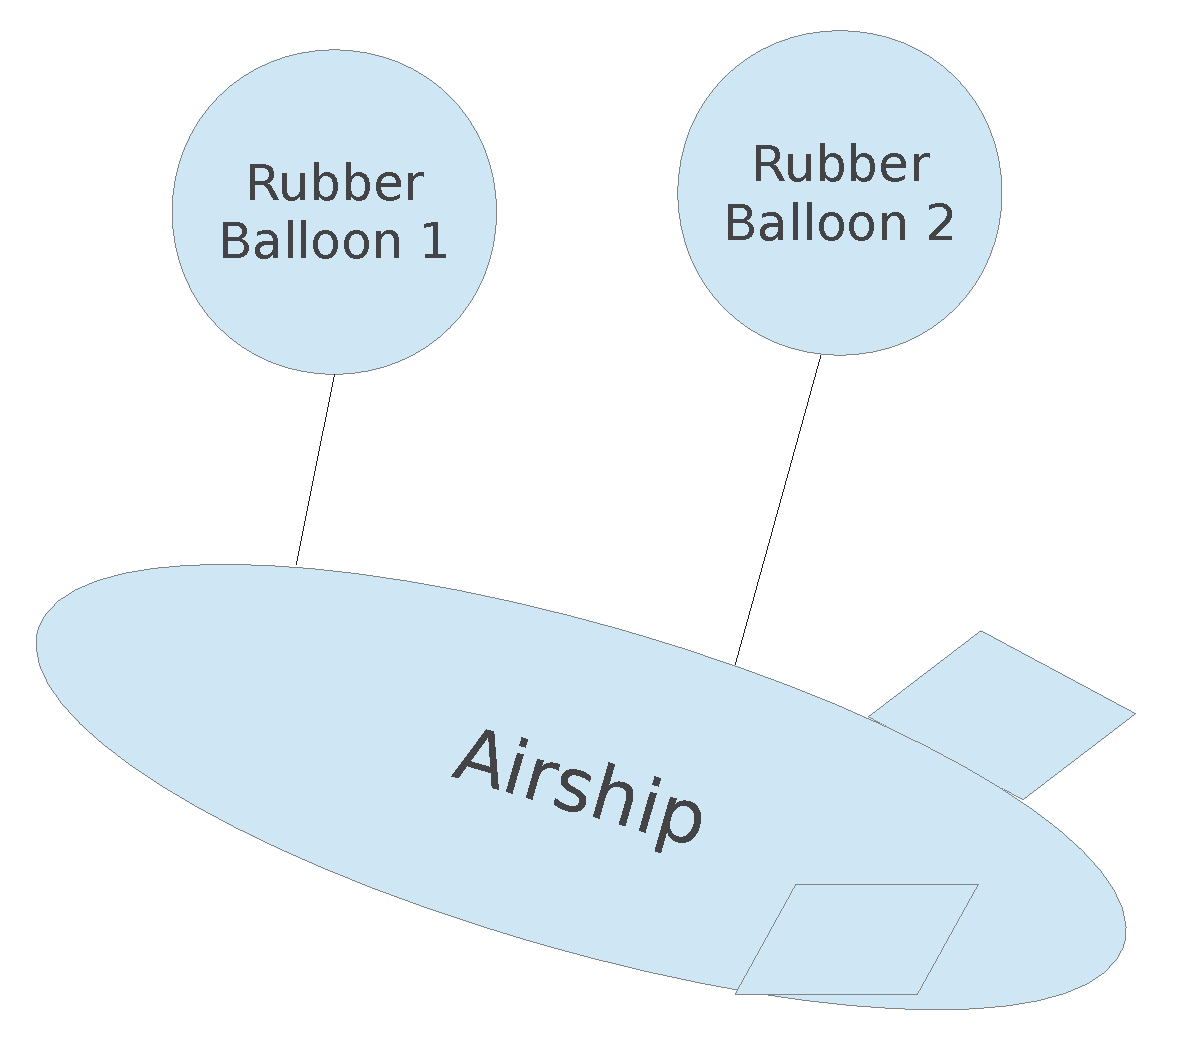
\includegraphics[scale=0.4]{airship.eps}
\caption{Airship with rubber balloon}\label{airship}
\end{figure}

The inflation of rubber balloon refers to the problem of large deformation\cite{Rivlin,Green Zerna,Green Shield,Atkins Rivlin}. To analyse or simulate this deformation, it is important to choose the material law\cite{Atkins Rivlin,Muller Struchtrup}. Mooney-Rivlin model is always used. Results from this model are compared with experimental data\cite{Atkins Rivlin}. M\"{u}ller and Struchtrup simulate the process of inflating a single balloon by mouth\cite{Muller Struchtrup}.

In fact the coefficients of elasticity in Mooney-Rivlin model depend on temperature due to its entropy induced elasticity\cite{Ingo}, this may influence the performance of rubber balloon. When we consider a long duration balloon at high altitude which would stay aloft over many diurnal cycles, the influence of temperature may not be neglected.

We studied the temperature effect of elasticity of rubber in this paper and found that it play an important role in the ascending process of rubber balloon, especially at high altitude.


\section{Mooney-Rivlin model}
  Since rubber is typical hyperelastic material, We choose the Mooney-Rivlin model as its constitute law.
  For a rubber balloon, the pressure equation is
  \begin{equation}\label{pressure}
  \Delta p= p_{in}-p_{out}
  \end{equation}
  The inner pressure $p_{in}$ can be calculated by ideal gas relation:
 \begin{equation}\label{idealgas}
  p_{in}=\frac{n R T}{\frac{4}{3} \pi r^3}
 \end{equation}
 $n$ is the number of moles of gas in the balloon, $R=8.3144 J\cdot K^{-1}\cdot mol^{-1}$ is the gas constant.
 The $\Delta p-r$ characteristic, which describes the dependence of pressure difference across the spherical rubber balloon's membrane on its radius, is non-monotonic, see Figure \ref{cha}. Its analytical form is
 \begin{equation}\label{prrelation}
  \Delta p(r)=2s_+\frac{t_0}{r_0}(\frac{r_0}{r}-(\frac{r_0}{r})^7)(1-\frac{s_-}{s_+}(\frac{r}{r_0})^2)
 \end{equation}

 \begin{figure}[!hbt]
  \centering
  % Requires \usepackage{graphicx}
    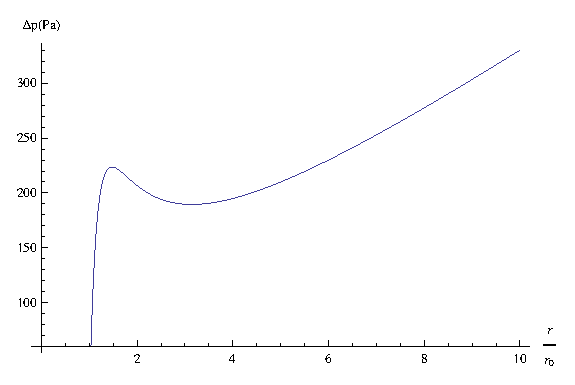
\includegraphics[scale=1]{cha.eps}\\
   \caption{Pressure radius characteristic}\label{cha}
 \end{figure}

 From(\ref{pressure}),(\ref{idealgas}), and (\ref{prrelation}), we obtain
 \begin{equation}\label{total}
  p_{out}(h)-\frac{n R T(h)}{\frac{4}{3} \pi r^3}+2s_+\frac{t_0}{r_0}(\frac{r_0}{r}-(\frac{r_0}{r})^7)(1-\frac{s_-}{s_+}(\frac{r}{r_0})^2)=0
 \end{equation}
 $t_0$ and $r_0$ are the unstretched thickness and radius of the balloon. $s_+$ and $s_-$ are the elastic coefficients. We notice that the atmospherical pressure and temperature is functions of altitude.
 We now study the ascending process of a rubber balloon with payload.
 The mass of payload $m_p=1.5kg$, the unstretched radius $r_0$ and thickness $t_0$ is given by the manufacturer, here, we set them $ 0.5m$ and $ 0.25mm$. With $r_0$, $t_0$, and the density of the rubber, we can work out the mass of the rubber balloon.
 We assume the radius at bursting to be $5m$.
 By setting $r$ to the initial inflation radius at $h=0$, we can obtain $n$. Then we can solve equation (\ref{total}) for $r$ at each altitude $h$.


\section{Modified Mooney-Rivlin model}
\subsection{Temperature effect}
 For rubber is the material with entropy-induced elasticity, the elastic coefficients $s_+$ and $s_-$ actually depend on temperature; their dependence on temperature is linear\cite{Ingo}. This means           %need citation
 \begin{equation}\label{s}
   \frac{s_+(T)}{s_+(T_0)}=\frac{s_-(T)}{s_-(T_0)}=\frac{T}{T_0}
 \end{equation}
 So equation (\ref{total}) needs some modification. It becomes to
 \begin{equation}\label{total1}
   p_{out}-\frac{n R T}{\frac{4}{3}\pi r^3}+2s_+(T)\frac{t_0}{r_0}(\frac{r_0}{r}-(\frac{r_0}{r})^7)(1-\frac{s_-(T_0)}{s_+(T_0)}(\frac{r}{r_0})^2)=0
 \end{equation}

Then the thermodynamic state of the inner gas is coupled with the strain or the stress of balloon. The behavior of rubber varies at different temperature, also at different altitude. The study here is to reveal how much of an effect this has on the ascending process.
\subsection{Comparison between Mooney-Rivlin models}
The typical value given in \cite{Ingo} for $s_+$ and $s_-$:
\begin{equation}\label{coefficient}
  s_+(300K)=300kPa, s_-(300K)=-30kPa
\end{equation}
Figure \ref{RA} shows the resulting graph of balloon radius versus height. As well as the Mooney-Rivlin model and the modified Mooney-Rivlin model, the graph also includes a purely theoretical non-restoring model, in which the balloon exerts no retractive elastic force at all ($\Delta p=0$, so the inner pressure is always equal to the atmospherical pressure).
\begin{figure}[!hbt]
  \centering
  % Requires \usepackage{graphicx}
  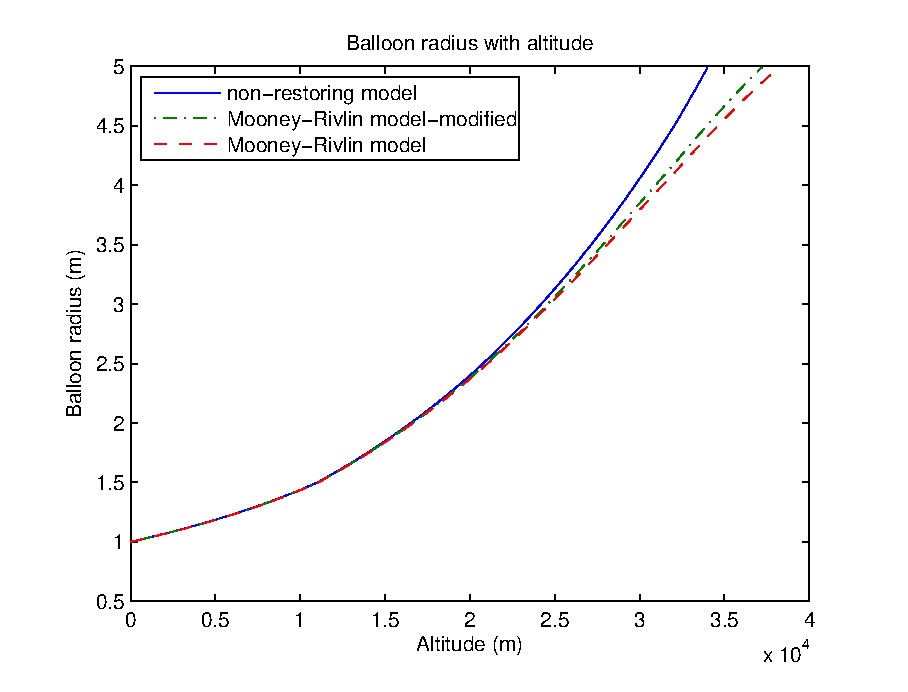
\includegraphics[scale=0.8]{RA.eps}\\
  \caption{Balloon radius with altitude}\label{RA}
\end{figure}


We have assumed the burst radius of the balloon as $5m$, This occurs at $34km$  for the non-restoring model, $38.2km$ for the Mooney-Rivlin model and $37.2km$ for the modified Mooney-Rivlin model with the provided parameters.
The result here suggests that the existence of elasticity increases the ceiling of the balloon though very limited. The difference between Mooney-Rivlin models is slight.

Figure \ref{PR} shows the pressure jump across the balloon membrane for each model.
\begin{figure}[!hbt]
  \centering
  % Requires \usepackage{graphicx}
  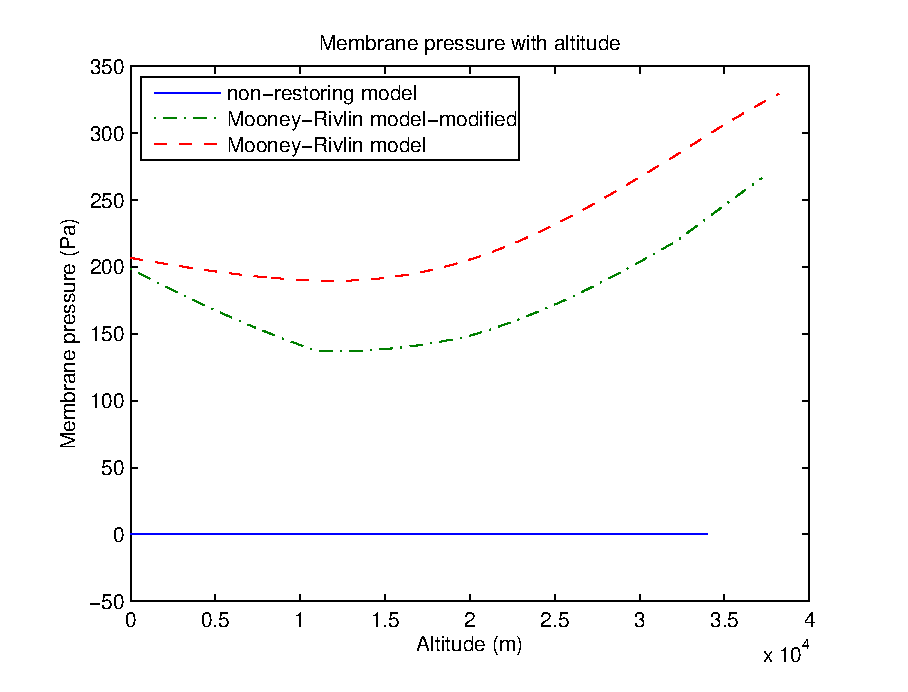
\includegraphics[scale=0.8]{PR.eps}\\
  \caption{Membrane pressure with altitude}\label{PR}
\end{figure}


For the balloon with the provided parameters here, it can be seen that the membrane pressure is of the order of $140-300 Pa$ throughout the flight envelope. This means that the difference in pressure between inside and outside is negligible at low altitudes(sea level pressure is about 101325 Pa). However, at high altitudes it may start to become significant. At 30 km the atmospheric pressure has fallen to $1197 Pa$  ; at 40 km it is $ 287 Pa$. This may lead some interesting phenomenon which we will see below.

We also get that the membrane pressure in modified Mooney-Rivlin model is always smaller than in Mooney-Rivlin model. This is because the temperature is lower at high altitude than sea level, then the restoring force decreases due to the entropy induced elasticity.

Lift is calculated by buoyancy minus gravity. Buoyancy is proportional to the product the volume of the balloon and the density of the atmosphere, while gravity contains three parts(payload, balloon and inner gas). The difference is very obvious when we plot the lift curves of different models, see Figure \ref{LA}.

\begin{figure}[!hbt]
  \centering
  % Requires \usepackage{graphicx}
  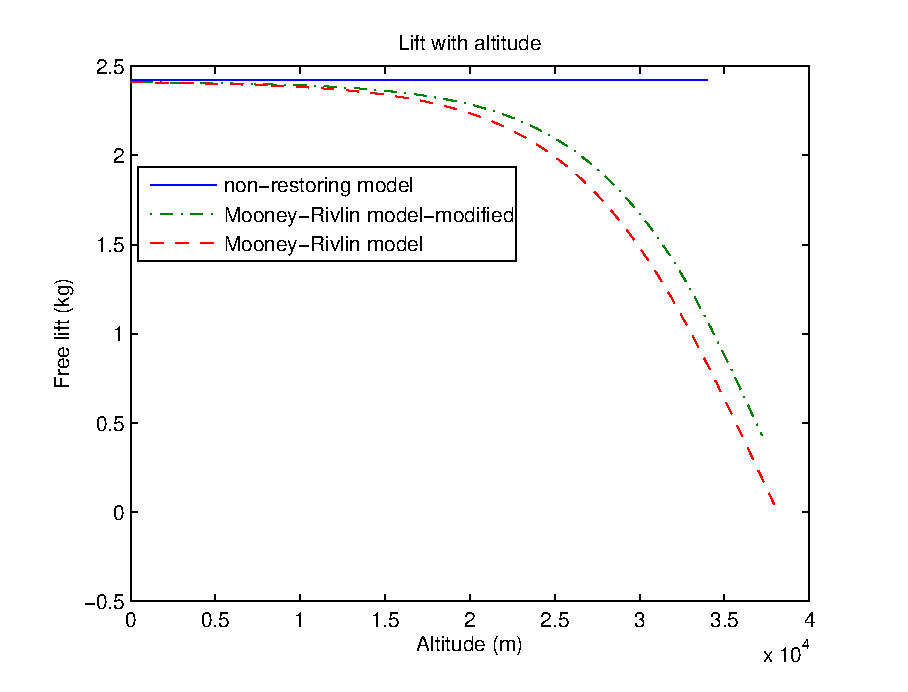
\includegraphics[scale=0.8]{LA.eps}\\
  \caption{Lift with altitude}\label{LA}
\end{figure}

Because there is no pressure jump across the membrane in the non-restoring model, the lift is constant. But this should be changed when we consider elasticity. The free lift decreases from $2.7kg$ to $1.0kg$ below as the balloon approaches its burst point in Mooney-Rivlin models. Though the balloon may still ascend, it is important when we need estimate whether the target altitude is achieved and assess the lift performance. We also get that the modified Mooney-Rivlin model has better lift performance than the normal one.

The ascent velocity was calculated based on the formula for terminal velocity:
\begin{equation}\label{LD}
  L=F_d= C_d\frac{\rho}{2} A v^2, v=\sqrt{\frac{2 L}{C_d \rho A}}
\end{equation}
here $C_d=0.47$ for a sphere, $A=\pi r^2$ is the cross-section area, and $\rho$ is the atmospherical density. It is easy to know lift $L$ and $\rho$ are functions of altitude. Then we plot the ascent velocity with altitude for each models(Figure \ref{VA}) .

\begin{figure}[!h]
  \centering
  % Requires \usepackage{graphicx}
  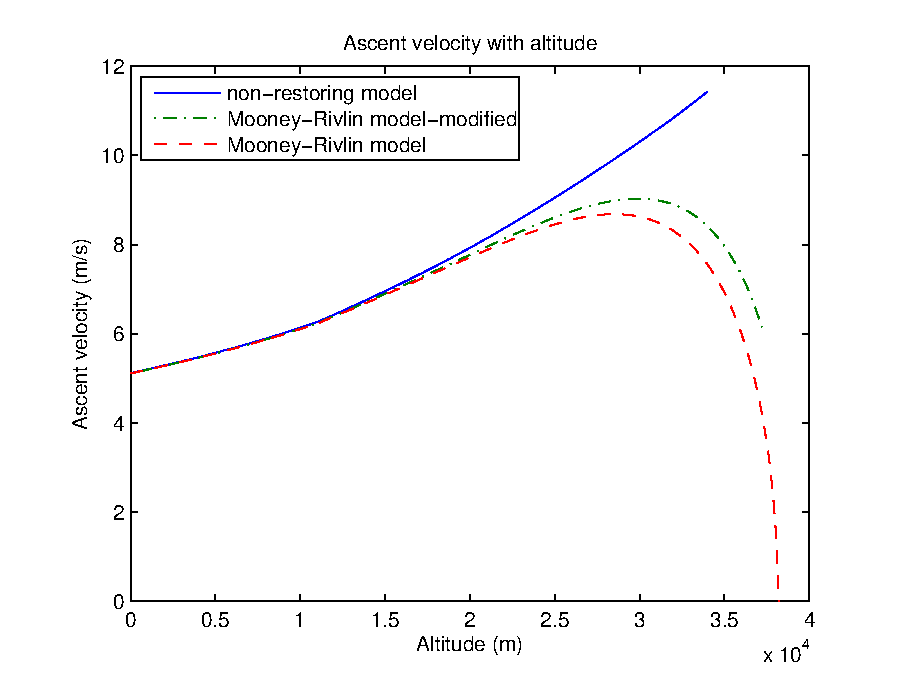
\includegraphics[scale=0.8]{VA.eps}\\
  \caption{Ascent velocity with altitude}\label{VA}
\end{figure}

The ascent velocity generally increases with height(below $30km$), but it decreases at high altitude(above $30km$) in Mooney-Rivlin models. When we consider the temperature effect in Mooney-Rivlin model, we found that the velocity is larger due to the better lift performance.


\subsection{Staying aloft}

Now we turn to consider another interesting phenomenon when the temperature effect of elasticity is taken account.


If the rubber balloon stay aloft at very high altitude(nearspace), say 80km, the atmospherical pressure is approximately $0 Pa$. Then equation (\ref{total1}) changes to
\begin{equation}\label{total2}
   - \frac{{n{R}T}}{{\frac{4}{3}\pi {r^3}}} + 2{s_ + }(T)\frac{{{t_0}}}{{{r_0}}}(\frac{{{r_0}}}{r} - {(\frac{{{r_0}}}{r})^7})(1 - \frac{{{s_ - }({T_0})}}{{{s_ + }({T_0})}}{(\frac{r}{{{r_0}}})^2}) = 0
\end{equation}
we can cancel $T$ in each term, then we get:
\begin{equation}\label{total3}
   - \frac{{n{R}}}{{\frac{4}{3}\pi {r^3}}} + 2\frac{{{s_ + }({T_0})}}{{{T_0}}}\frac{{{t_0}}}{{{r_0}}}(\frac{{{r_0}}}{r} - {(\frac{{{r_0}}}{r})^7})(1 - \frac{{{s_ - }({T_0})}}{{{s_ + }({T_0})}}{(\frac{r}{{{r_0}}})^2}) = 0
\end{equation}

It suggests that the balloon's radius $r$ is independent with temperature, the balloon will keep its shape when the balloon's temperature changed, this is important when we consider a balloon that is capable of staying aloft for half a year at high altitude. At night the temperature of the lifting gas cools, while the temperature rises caused by solar heating during the day. These are called "supercool" and "superheat". From the equation above, though the temperature varies during the diurnal cycles, the balloon will keep its volume, so the residence altitude. This will be a great advantage when we use rubber balloon as the High Altitude Long Duration aerostat.


\section{Conclusion}
The ascending process of a rubber balloon has been studied. Due to the entropy induced elasticity, the elastic behavior of rubber varies at different temperature. We set rubber as material of a modified Mooney-Rivlin relation, and we found that the temperature effect of elasticity plays an important role in ascending process.
We also show the interesting phenomenon that the balloon will keep its height when temperature changes at high altitude. This fact may has great significance when we develop a high altitude long duration balloon.

But the dependence of elastic coefficient of rubber on temperature is rather complex, and the nature of them is still not clear\cite{Shedd Ingersol}. In fact, from the experiment the coefficient $s_-$ is always increasing more slowly than the absolute temperature\cite{Shumskaya}. Even more, the material of rubber balloons is not strictly a Mooney-Rivlin model. All these make it more difficult to predict the performance of  rubber balloon.
But in any case, the temperature effect of elasticity  of rubber balloon should be considered in the extreme environment.


\begin{thebibliography}{99}
\setlength{\parskip}{0pt}  %����֮�����ֱ����


\bibitem{Rivlin}Rivlin R.S. Large Elastic Deformations of Isotropic Materials. II. Some Uniqueness Theorems for Pure, Homogeneous Deformation. Phil. Trans. R. Soc. Lond. A  240, 491-508 (1948).
\bibitem{Green Zerna}Green A.E. and Zerna E. XXVI. Theory of elasticity in general coordinates., Philosophical Magazine Series 7, 41, 315, 313-336 (1950)
\bibitem{Green Shield} Green A.E. and Shield, R.T. Finite Elastic Deformation of Incompressible Isotropic Bodies. Proc. R. Soc. Lond. A 202, 407-419 (1950).
\bibitem{Atkins Rivlin}Atkins J.E. and Rivlin R.S. Large Elastic Deformations of Isotropic Materials. IX. The Deformation of Thin Shells, Phil. Trans. R. Soc. Lond. A 244, 505-531 (1951).
\bibitem{Muller Struchtrup}M\"{u}ller I. and Struchtrup H. Inflating a Rubber Balloon. Mathematics and Mechanics of Solids, 7, 569-577 (2002).
\bibitem{Ingo} M\"{u} I. and Strehlow P. Rubber and rubber balloons: paradigms of thermodynamics. Lecture Notes in Physics, Springer, 2004
\bibitem{Shedd Ingersol}Shedd J.C. and Ingersol R.L. The Elastic Modulus and Elastic Limit of Rubber and Theri Relation to Change of Temperature. Phys. Rev. (Series I) 19, 107-116 (1904).
\bibitem{Shumskaya} Shumskaya A.G., Priss L.S., and Popov V.F. Temperature Dependence of Elastic Constants of Rubber. J.Polymer SCI.: Symposium, 53, 219-230 (1975).
\end{thebibliography}
\end{document}
